\section{Step-by-Step Simulation}
\label{sec:analysis:step-by-step}
\label{sec:modeling:step-by-step}

UPPAAL provides a model simulations tool, allowing the user to generate model
executions by selecting each transition to take. This can be used to assert
that a particular execution is indeed a valid trace of the model. It also helps
to understand and debug the model. Furthermore, when using UPPAAL's model
checker, the generated counter-examples can be explored in the
step-by-step simulation tool. This helps understanding exactly what allowed the
counter-example to be reached.

It should be noted that using the extremum operators (\texttt{sup} or
\texttt{inf}, described in Section~\ref{sec:uppaal_queries}) in a model
checking query never generates a counter-example: the property is always
considered as having been verified. The resulting value is simply given to the
user in the form of a pop-up dialog. To obtain a trace in the step-by-step
simulator that would yield this extremum, the user has to perform a new
verification. Indeed, a solution is then to ask UPPAAL to verify that the
system never reaches a state in which the target clock or variable has the
extremum value. This will generate a counter example, and thus one trace for
which the model reaches this value.

\begin{figure}[hbt!]
\begin{center}
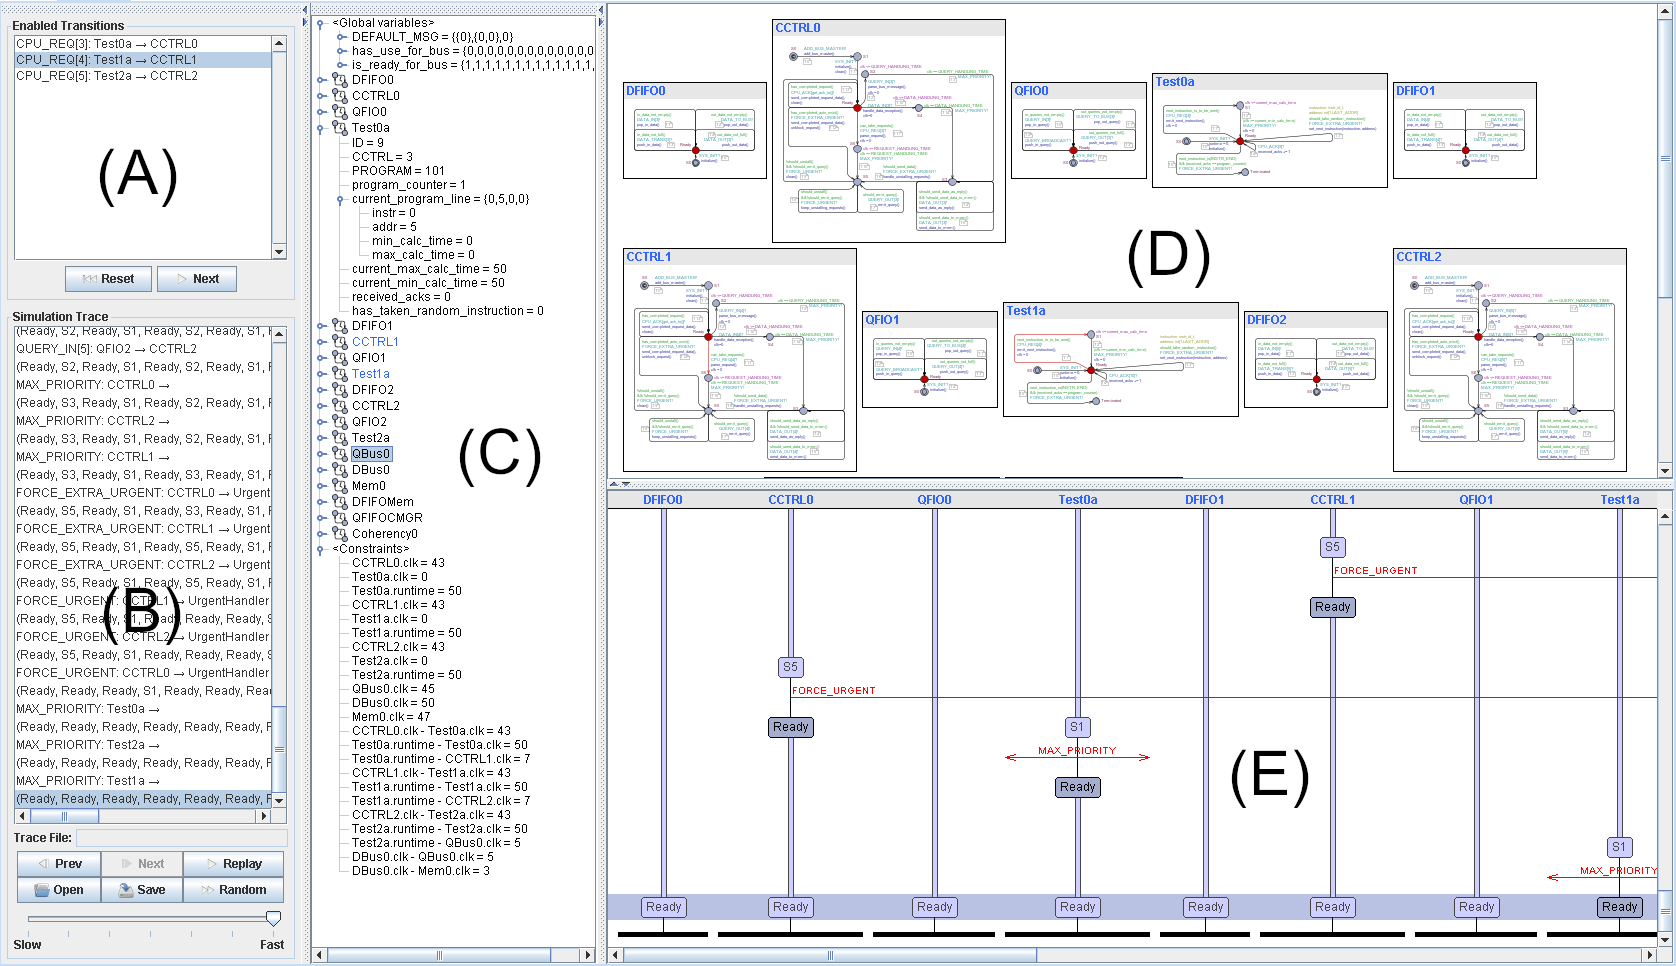
\includegraphics[width=\textwidth]{\chapterdirectory/figure/step-by-step-labels.png}
\end{center}
\caption{UPPAAL Step-by-Step Simulation Interface}
\label{fig:UPPAAL:step-by-step}
\end{figure}

Figure~\ref{fig:UPPAAL:step-by-step} shows UPPAAL's step-by-step simulation
interface. Using this, the user is able to simulate an execution of the model
for which they are able to decide the order of any transition: the available
transitions in the current state are displayed in \lstinline!(A)!; those
that were previously taken are shown in \lstinline!(B)! and the system can be
reverted to any of them with a simple click; the valuation of each variable and
the current clock constraints are displayed in \lstinline!(C)!; the current
location of each automaton is displayed in \lstinline!(D)!; and the
synchronizations that have occurred so far are displayed in \lstinline!(E)!.
